\subsection{综合工作负载评估}
\label{subsec:synthetic}


我们使用一组文件生成一个合成数据集,每个文件都包含全局非重复块。 默认情况下,我们将文件大小设置为 2\,GB(Exp\#2 除外,我们在其中对 消息锁加密(MLE) 密钥生成性能进行了压力测试)。 客户端通过云上传或下载文件。 为了避免磁盘 I/O 对性能的影响,我们将文件数据存储在内存中而不是磁盘上(Exp\#5 除外,我们在实云部署中处理磁盘上的文件)。 我们绘制了 10 次运行的平均结果。 我们还将 \textit{ Student's t-Distribution} 的 95\% 置信区间包含在条形图中(为简洁起见,我们将它们从折线图中排除)。


\begin{figure}[!htb]
\centering
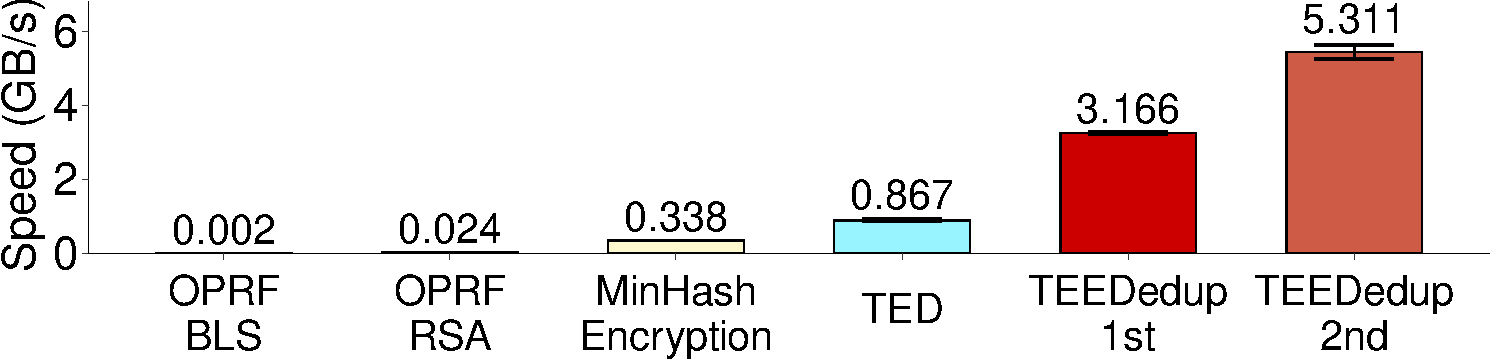
\includegraphics[width=\textwidth]{pic/sgxdedup/expa2_keyGenPerformance.pdf}
\vspace{-12pt}
\caption{(Exp\#1) Single-client 消息锁加密(MLE) key generation.}
\label{fig:keygen-comparison}
\end{figure}

\begin{figure}[!htb]
  \begin{minipage}[t]{0.47\textwidth}
  \centering
  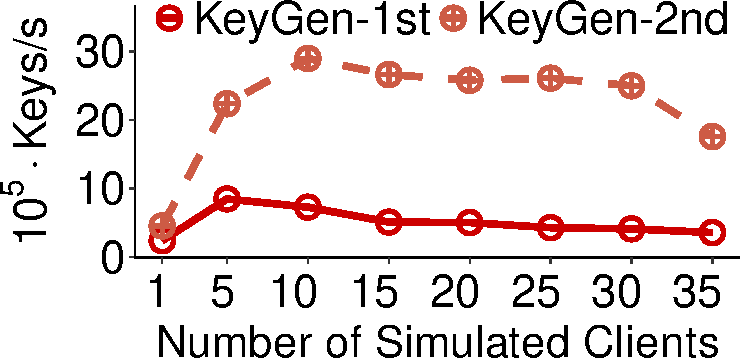
\includegraphics[width=\linewidth]{pic/sgxdedup/expa3_keyScale_performance_number_multiThread.pdf}
  \vspace{-12pt}
  \caption{(Exp\#2) Multi-client 消息锁加密(MLE) key generation.}
  \label{fig:exp-keygen-scalability}
  \end{minipage}%
  \hspace{0.2in}
  \begin{minipage}[t]{0.47\textwidth}
  \centering
  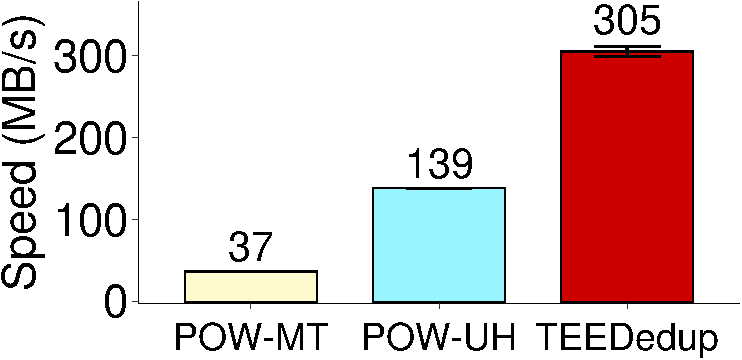
\includegraphics[width=\linewidth]{pic/sgxdedup/expa4_powPerformance.pdf}
  \vspace{-12pt}
  \caption{\small(Exp\#3) Computational PoW.}
  \label{fig:pow-comparison}
  \end{minipage}%
  \vspace{-6pt}
\end{figure}


\paragraph{Exp\#1(单客户端 消息锁加密(MLE) 密钥生成)。} 我们在两轮中评估 消息锁加密(MLE) 密钥生成。首先,客户端通过 Rabin 指纹 (\S\ref{sec:implementation}) 创建 2\,GB 文件的明文块并发出 消息锁加密(MLE) 密钥生成请求。然后它为不同的 2\,GB 文件的块重复 消息锁加密(MLE) 密钥生成过程。不同之处在于第二轮使用预先计算的掩码生成 消息锁加密(MLE) 密钥 (\S\ref{subsec:encryption})。

我们将 \sysnameS 的单客户端 消息锁加密(MLE) 密钥生成速度与最新技术进行了比较。我们考虑两种基于 OPRF 的密钥生成方法,即 \textit{ OPRF-BLS} \cite{armknecht15} 和 \textit{ OPRF-RSA} \cite{bellare13b},它们实现了 OPRF 原语(\S\ref{subsec:encrypted-dedup})分别基于盲 BLS 和盲 RSA 签名。我们还考虑了两种宽松的密钥生成方法,即 \textit{ MinHash encryption} \cite{qin17} 和 \textit{ TED} \cite{li20b},它们以存储效率和安全性换取性能。具体来说,MinHash 加密使用 OPRF-RSA 在每个段的基础上生成 消息锁加密(MLE) 密钥,其中平均段大小配置为 1\,MB。 TED 根据块的短散列的基于草图的频率计数为每个块生成 消息锁加密(MLE) 密钥(参见 \cite{li20b} 中的 \S3.3)。

图~\ref{fig:keygen-comparison} 显示了结果。 \sysnameS 通过避免 OPRF-BLS、OPRF-RSA 和 MinHash 加密中昂贵的密码原语以及 TED 中的频率计数计算,优于所有基线方法。它的第一轮分别比 OPRF-BLS 和 OPRF-RSA 实现了 1,583$\times$ 和 131.9$\times$ 的加速。与 MinHash 加密和 TED 相比,加速分别为 9.4$\times$ 和 3.7$\times$,尽管后两者牺牲了存储效率和安全性。第二轮投机加密将第一轮的 消息锁加密(MLE) 密钥生成速度提高了 67.8\%。



\paragraph{Exp\#2(多客户端 消息锁加密(MLE) 密钥生成)。} 我们评估多客户端 消息锁加密(MLE) 密钥生成。对于压力测试,我们配置了一台运行多个线程的机器,每个线程都模拟一个客户端,同时向密钥管理器(在不同的机器上运行)发出 消息锁加密(MLE) 密钥生成请求。回想一下,密钥安全区中预先计算的掩码可用于有效处理最多 11.25GB 的数据 (\S\ref{subsec:encryption})。为了在第二轮中为每个模拟客户端启用推测性加密,我们将每个线程配置为生成 40,960 个指纹(即 320 个,8 个 KB 块的 MB 原始数据),并将密钥安全区配置为同等地预先计算掩码每个模拟客户端在第一轮密钥生成之后。我们在处理来自所有模拟客户端的所有 消息锁加密(MLE) 密钥生成请求时测量 \textit{ aggregate} 消息锁加密(MLE) 密钥生成速度。

图~\ref{fig:exp-keygen-scalability} 展示了结果。两轮的总密钥生成速度最初随着模拟客户端的数量而增加。在高峰期,第一轮和第二轮分别为 5 个和 10 个模拟客户端实现了 $8.5\times 10^5$\,keys/s 和 $29\times 10^5$\,keys/s。在十个客户端之后,由于加重的上下文切换开销,聚合速度下降。平均而言,第二轮的投机加密比第一轮实现了 4.4$\times$ 的聚合密钥生成加速。


\paragraph{Exp\#3 (Computational PoW).} 我们评估 PoW 的性能。我们考虑一个对 2GB 文件执行 PoW 的客户端。客户端从文件中创建明文块,加密每个明文块,并向云端发出 PoW 请求。我们根据客户端(PoW安全区对密文块执行指纹识别并签署结果指纹)和云(验证数据的真实性)中所有块的总计算时间来测量 \textit{ 计算 PoW 速度}指纹);请注意,我们在速度计算中排除了客户端和云端之间的网络传输时间(我们在附录中的 Exp\#11 中考虑了网络传输时间)。

我们将 \sysnameS 与两种最先进的 PoW 方法进行比较:(i) \textit{ PoW-MT} \cite{halevi11}(又名 \cite{halevi11} 中的基本版本), PoW 方法使用纠删码对块进行编码,并在 PoW 的编码内容上构建 Merkle 树; (ii) \textit{ PoW-UH} \cite{xu13},它建立在通用散列之上,但以安全性换取性能。为了公平比较,我们自己在 C++ 中实现了 PoW-MT 和 PoW-UH。请注意,有改进的 PoW 方法 \cite{halevi11},但它们会因低内存使用而产生更高的性能开销。


图~\ref{fig:pow-comparison} 显示了结果。 \sysnameS 显着优于 PoW-MT,因为它避免了客户端中的擦除编码和 Merkle 树构造,以及云中基于 Merkle 树的验证。 它比 PoW-MT 实现了 8.2$\times$ 的加速。 它还比 PoW-UH 实现了 2.2$\times$ 的加速。


\begin{figure}[t]
  \centering
  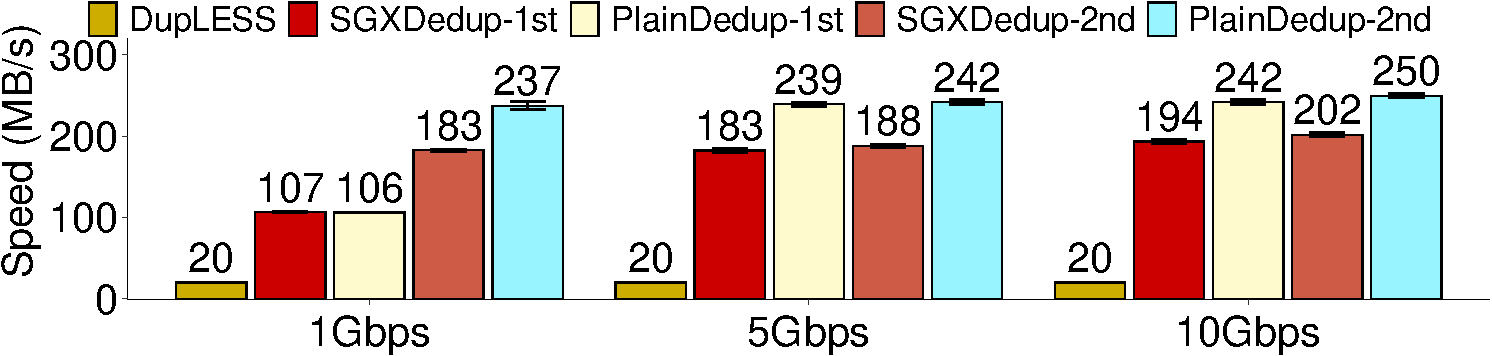
\includegraphics[width=0.6\textwidth]{pic/sgxdedup/upload_network_speed_bar.pdf} \ \ 
  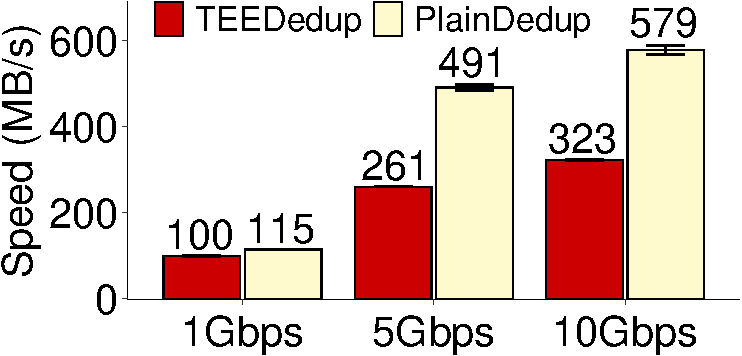
\includegraphics[width=0.3\textwidth]{pic/sgxdedup/download_network_speed_bar.pdf}
  \vspace{-3pt}\\
    \hspace{1.1in} {\small (a) Upload} \hspace{1.9in}
  {\small (b) Download}
  \vspace{-6pt}\\
  \caption{(Exp\#4) Single-client uploads and downloads. We exclude the second upload speed of {\em DupLESS} (which has the same performance in two uploads) and the download speed of {\em DupLESS} (which is identical to that of  \sysnameS).}
  \label{fig:singleClientThroughput}
\end{figure}

\begin{figure}[t]
  \centering
  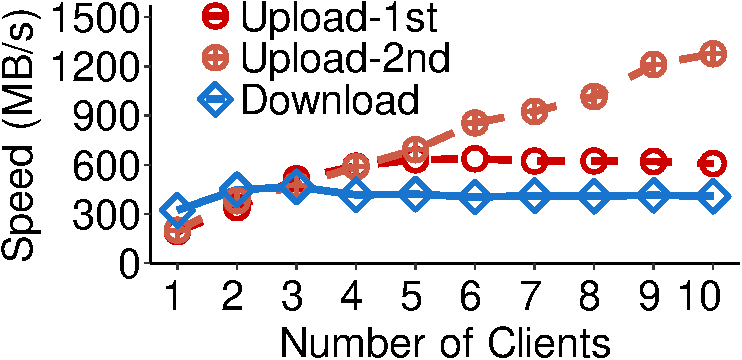
\includegraphics[width=0.6\textwidth]{pic/sgxdedup/expb1_multiple_client.pdf}  
  \caption{(Exp\#6) Multi-client uploads and downloads.}
  \label{fig:multiClientThroughput}
\end{figure}

\paragraph{Exp\#4 (Single-client uploads and downloads).} 我们考虑单个客户端,并将 \sysnameS 的上传和下载性能与两个基线系统进行比较:(i) \textit{ PlainDedup},禁用 \sysnameS 的密钥生成、加密和PoW操作,从而实现基于数据源的重复数据删除,无需任何安全保护; (ii) \textit{ {\em DupLESS}} \cite{bellare13b},它通过 OPRF-RSA 生成每块 消息锁加密(MLE) 密钥,执行加密并将所有密文块上传到云以进行重复数据删除。由于 {\em DupLESS} 的原始实现不提供重复数据删除存储后端(假设使用了 Dropbox),我们根据 \cite{bellare13b} 中描述的设计在 C++ 中实现 {\em DupLESS}。请注意,PlainDedup 基于未加密的文件元数据检索文件,并且不同于加密重复数据删除系统中的两轮下载(即 \sysnameS 和 {\em DupLESS});在后者中,客户端首先下载并解密文件元数据,然后下载块以重建文件 (\S\ref{subsec:encrypted-dedup})。

我们分三个步骤评估上传和下载速度: (i) 客户端首先上传 2\,GB 文件; (ii) 客户端重新启动,然后上传另一个与前一个相同的 2\,GB 文件; (iii) 客户端下载文件。请注意,第二次上传执行基于数据源的重复数据删除(对于 PlainDedup 和 \sysnameS),并利用预先计算的掩码来加速密钥生成(仅适用于 \sysnameS)。

图~\ref{fig:singleClientThroughput}(a) 显示了由 {\tt trickle} \cite{eriksen05} 控制的不同网络带宽的上传速度。第一次上传,当网络带宽为 1\,Gbps 时,\sysnameS (106.6\,MB/s) 和 PlainDedup (106.2\,MB/s) 的上传速度均受网速约束,而性能{\em DupLESS} (20.1\,MB/s) 的瓶颈是基于 OPRF-RSA 的密钥生成 (Exp\#1)。当网络带宽增加到 10\,Gbps(默认)时,\sysnameS 和 PlainDedup 的上传速度分别达到 193.6\,MB/s 和 242.0\,MB/s,而 {\em DupLESS} 的上传速度稳定在 20.0\, MB/秒。对于第二次上传,由于其密钥生成性能瓶颈,{\em DupLESS} 达到了与第一次上传相同的速度。 \sysnameS 和 PlainDedup 的上传速度受网络带宽的影响较小,因为它们不需要传输数据。平均而言,\sysnameS 在第一次和第二次上传中分别比 {\em DupLESS} 实现了 8.1$\times$ 和 9.6$\times$ 的加速。即使与不安全的 PlainDedup 相比,\sysnameS 也只会导致相应的上传速度下降约 17.5\% 和 21.4\%。开销来自 \sysnameS 的安全机制,包括密钥生成、加密和 PoW。

图~\ref{fig:singleClientThroughput}(b) 显示了下载速度。随着网络带宽增加到 10\,Gbps,\sysnameS 和 {\em DupLESS} 均达到 323.1\,MB/s,比 PlainDedup 下降了 44.2\%。原因是他们连续检索和解密文件元数据,然后下载密文块。

\paragraph{Exp\#5(真实云上传和下载)。} 我们现在扩展 Exp\#4 并评估真实云部署中的上传和下载速度。具体来说,我们将客户端和密钥管理器部署在我们的局域网测试平台(\S\ref{sec:evaluation})中,并通过互联网将客户端连接到\textit{ 阿里云},我们在其中租用了一个虚拟机\textit{ ecs.c6e.xlarge} 运行云。云机配备四核3.2GHz CPU(其主机平台为Intel Xeon Cascade Lake Platinum 8269CY),8GB内存。我们以 \textit{ Alibaba General Purpose NAS} 作为存储后端来挂载云。 NAS 可以实现高达 20000\,IOPS 的 4\,K 次随机读写。

我们使用磁盘上的数据文件进行上传(与 Exp\#4 相对,后者在上传之前将文件加载到客户端的内存中),并允许云端将接收到的数据文件存储在 NAS 中。我们还使用 {\tt scp} 将整个数据文件(即 2\,GB)从客户端上传到云端,以提供互联网环境下的数据传输基准。


Table~\ref{tab:real-cloud} 显示了结果。在第一次上传时,所有系统的性能(\sysnameS 为 11.4\,MB/s,PlainDedup 为 11.6\,MB/s,{\em DupLESS} 为 10.8\,MB/s)受限于 Internet 带宽(11.9\,MB/ s)。在第二次上传中,\sysnameS 实现了 104.3\,MB/s,与 {\em DupLESS} 相比加速了 9.7$\times$,与 PlainDedup 相比下降了 13.2\%。请注意,性能差异比 Exp\#4 中的要小,因为 \sysnameS 和 PlainDedup 现在受客户端磁盘 I/O 的限制。在下载中,这三个系统的性能再次受到 Internet 带宽的限制,而 \sysnameS 和 {\em DupLESS} 由于它们的串行检索和解密(Exp\#4),将 PlainDedup 的下载速度降低了 10.6\%。

\begin{table}[t]
\small
\centering
\renewcommand{\arraystretch}{1.05}
\begin{tabular}{|c|c|c|c|}
\hline
{\bf Approach} & {\bf First Upload} & {\bf Second Upload} & {\bf Download} \\
\hline
\hline
Transfer & \multicolumn{3}{c|}{11.9 $\pm$ 0.03} \\  
\hline
\hline
\sysnameS & 11.4 $\pm$ 0.3 & 104.3 $\pm$ 1.2 & 10.1 $\pm$ 0.1 \\ 
\hline
PlainDedup & 11.6 $\pm$ 0.1 & 120.1 $\pm$ 1.4 & 11.3 $\pm$ 0.3 \\
\hline
{\em DupLESS} & \multicolumn{2}{c|}{10.8 $\pm$ 0.2}  & 10.1 $\pm$ 0.1 \\
\hline
\end{tabular}
\vspace{-3pt}
\caption{(Exp\#5) Real-cloud upload and download (unit: MB/s).} 
\label{tab:real-cloud}
\vspace{-6pt}
\end{table}

\paragraph{Exp\#6(多客户端上传和下载)。}我们现在考虑同时发布上传/下载的多个客户端。我们专注于 \sysnameS,并将密钥安全区配置为在第一次上传后为每个客户端同等地预先计算掩码。我们将网络带宽固定为 10\,Gbps,并评估所有客户端完成上传/下载的 \textit{ aggregate} 上传和下载速度。

图~\ref{fig:multiClientThroughput} 显示了多达 10 个客户端的结果。第二轮的总上传速度随着客户端数量的增加而增加,达到1277.1\,MB/s。另一方面,由于客户端之间的写竞争,第一轮的总上传速度增加了七个客户端的 637.0MB/s,随后下降到 10 个客户端的 620.3MB/s。同样,由于多个客户端的读取竞争,总下载速度最终下降到 408.8\,MB/s。

\paragraph{Exp\#7(时间分解)。} 我们提供 \sysnameS 的时间分解来研究不同步骤的性能。假设key enclave已经启动,我们关注单个客户端的初始化和上传过程。初始化过程引导客户端的 PoW 安全区。上传过程包括以下步骤: (i) \textit{ chunking},将输入文件划分为明文块; (ii) \textit{ fingerprinting-p},计算明文块的指纹; (iii) \textit{ key generation},从密钥安全区生成 消息锁加密(MLE) 密钥; (iv) \textit{ encryption},加密明文块; (v) \textit{ fingerprinting-c},PoW安全区计算密文块的指纹; (vi) \textit{ 签名},PoW安全区计算指纹的签名; (vii) \textit{ 验证},其中云验证接收到的指纹的真实性; (viii) \textit{ deduplication},云检测重复的密文块并通知客户端; (ix) \textit{ transfer},上传非重复密文块和文件元数据。


\begin{table}[t]
\small
\centering
\setlength{\tabcolsep}{5pt}
\renewcommand{\arraystretch}{1.05}
\begin{tabular}{|c|c|c|c|}
\hline
  \multicolumn{2}{|@{\,}c|}{\textbf{Procedure/Step}} & \multicolumn{1}{l|}{\hspace{.5em}\textbf{First
  Upload}} &
\multicolumn{1}{c|}{\textbf{Second Upload}}                                                   \\ \hline \hline
\multicolumn{2}{|@{\,}c|}{Initialization}                   & 9.38 $\pm$
2.72\,s                                       & 0.80 $\pm$ 0.004\,s                       \\ \hline
\hline
                       \multicolumn{2}{|c|}{Chunking}                                 &
\multicolumn{2}{c|}{3.77 $\pm$ 0.15\,ms }                                                \\ \hline 
\multicolumn{2}{|c|}{Fingerprinting-p}
                                                           &
\multicolumn{2}{c|}{3.24 $\pm$ 0.28\,ms}                                                  \\ \hline
\multicolumn{2}{|c|}{Key generation}                     &
0.31 $\pm$ 0.01\,ms                           & 0.18
$\pm$ 0.01\,ms                                                                            \\ \hline
\multicolumn{2}{|c|}{Encryption} &
\multicolumn{2}{c|}{2.47 $\pm$ 0.10\,ms }                                                 \\ \hline
\multirow{3}{*}{PoW}  & Fingerprinting-c & \multicolumn{2}{c|}{3.28 $\pm$ 0.01\,ms }                                                 \\ \cline{2-4}
                      & Signing & \multicolumn{2}{c|}{0.01 $\pm$ 0.00004\,ms }                                                                                 \\ \cline{2-4}
                      & Verification & \multicolumn{2}{c|}{0.005 $\pm$ 0.00003\,ms } \\ \hline
                      \multicolumn{2}{|c|}{Deduplication}  & \multicolumn{1}{c|}{0.38 $\pm$ 0.03\,ms } & 0.48 $\pm$ 0.03\,ms  \\ \hline
                      \multicolumn{2}{|c|}{Transfer}  & \multicolumn{1}{c|}{1.29 $\pm$ 0.09\,ms } & 0.05 $\pm$ 0.01\,ms  \\ \hline
\end{tabular}
\vspace{-3pt}
\caption{(Exp\#7) Time breakdown per 1\,MB of file data processed: fingerprinting-p and fingerprinting-c are operated on plaintext and ciphertext chunks, respectively.}
\label{tab:system-breakdown}
\vspace{-6pt}
\end{table}

表~\ref{tab:system-breakdown} 显示结果(每 1\,MB 处理的文件数据)。初始化过程在第一次上传时非常耗时,因为它需要联系Intel认证服务以检查 PoW 安全区的完整性。客户端再次重启时,不再需要执行远程认证,首轮设置时间减少91.5%。请注意,初始化过程的时间开销可以在多次上传和下载中分摊。


密钥生成步骤是高效的,最多占用整个上传时间的 2.1\%。通过推测性加密,\sysnameS 进一步将第一次上传的密钥生成时间减少了 41.9\%。此外,整个 PoW 步骤占用了总上传时间的 24.4\%,而 PoW 中的主要计算是密文块的指纹识别,这对于在加密重复数据删除中查找重复项是必要的。通过轻量级的签名和验证步骤(最多占用总上传时间的 0.1\%),我们可以保护基于数据源的重复数据删除免受侧通道攻击,同时将首次上传的传输时间减少 96.1\%。

\paragraph{Exp\#10(指纹批量大小的影响)。} 我们首先使用 Exp\#1 的方法来评估指纹批量大小对密钥生成速度的影响。图~\ref{fig:exp-keygen-breakdown}(a) 显示了两轮密钥生成速度与指纹批量大小的关系。当我们将指纹批量大小从 1 更改为 $2^{15}$ 时,第一轮和第二轮的密钥生成速度从 0.0086\,GB/s 增加到 3.3\,GB/s 和从 0.0091\,GB/ s 到 6.5\,GB/s,分别。图~\ref{fig:exp-keygen-breakdown}(b) 进一步显示了客户端的计算时间分解以及每个生成 1MB 数据的 消息锁加密(MLE) 密钥的密钥安全区。客户端的消耗时间随着指纹批量大小而减少,因为更大的批量大小意味着要为所有指纹批次计算的 MAC 更少。此外,key安全区的消耗时间在第一轮从 2.0\,ms 减少到 0.2\,ms,在第二轮从 1.8\,ms 减少到 0.1\,ms。原因是较大的指纹批大小避免了对 key安全区的过多 ECall,并减少了 CPU 上下文切换开销。


\begin{figure}
\centering
\begin{tabular}{@{\ }c@{\ }c}
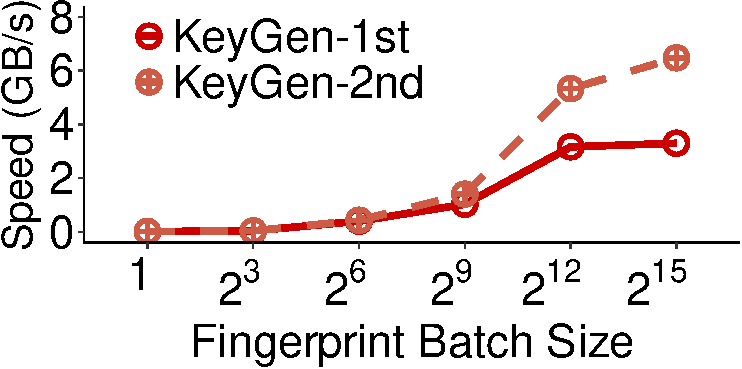
\includegraphics[width=0.48\textwidth]{pic/sgxdedup/expa2_keyEnclaveBatchSize_Performance_overall.pdf}                                         &
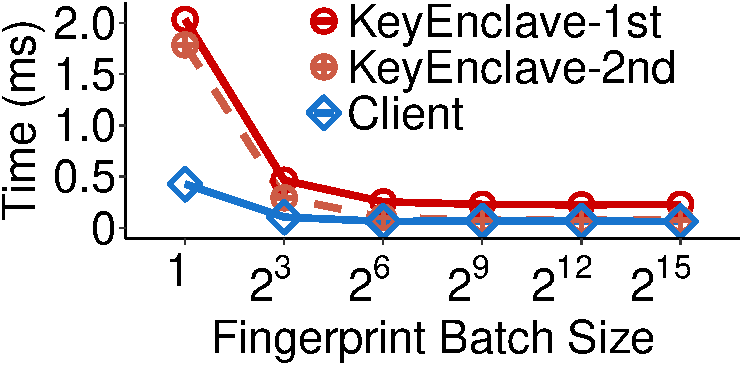
\includegraphics[width=0.48\textwidth]{pic/sgxdedup/expa2_keyEnclaveBatchSize_Performance_1st.pdf}                                               \\
\mbox{\parbox{0.48\textwidth}{\small (a) Key generation speed vs. fingerprint batch size}} &
\mbox{\parbox{0.48\textwidth}{\small (b) Computational time per generating 消息锁加密(MLE) keys of 1\,MB data}}
\end{tabular}
\caption{(Exp\#10) Impact of fingerprint batch size to key generation performance.}
\label{fig:exp-keygen-breakdown}
\end{figure}


\paragraph{Exp\#11 (Impact of ciphertext batch size).} 我们现在评估密文块批大小对 \sysnameS 的 PoW 性能的影响。与 Exp\#3 中考虑的计算 PoW 速度相反,我们测量 \textit{ 有效 PoW 速度},作为文件大小(即 2\,GB)与从 PoW安全区开始的总时间的比率计算密文块的指纹,直到云验证所有指纹。我们禁用客户端的上传操作和云端的重复数据删除操作,以减轻性能噪音。

图~\ref{fig:exp-pow-impact}(a) 显示了有效 PoW 速度与不同批量大小的关系。我们看到有效 PoW 速度随着密文批量大小从 6.2\,MB/s 到 360.9\,MB/s 的增加而增加。图~\ref{fig:exp-pow-impact}(b) 显示了 PoW 安全区和云在 PoW 中每次操作 1\,MB 数据时的相应计算时间。云的消耗时间很低(例如,低于 0.05\,ms),而 PoW安全区的时间随着批量大小从 4.1\,ms 减少到 2.7\,ms,因为减少了上下文切换开销(见 Exp \#10)。请注意,即使批量密文块的总大小超过 EPC 大小,PoW安全区仍保持高计算性能,因为它不需要将数据内容复制到安全区(\S\ref{sec:implementation})。

\begin{figure}[t]
\centering
\begin{tabular}{@{\ }c@{\ }c}
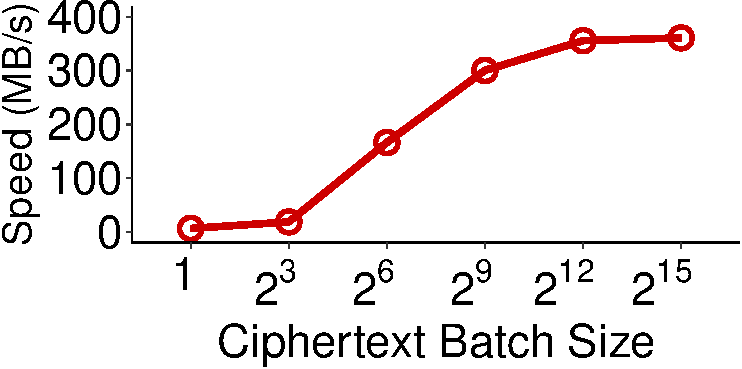
\includegraphics[width=0.48\textwidth]{pic/sgxdedup/expa4_powBatchSize_overall.pdf} &
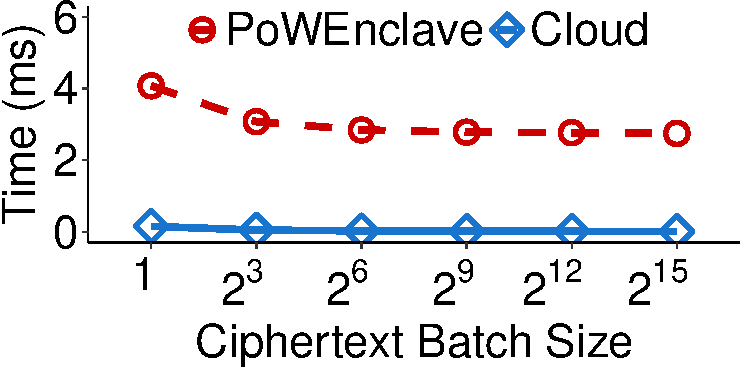
\includegraphics[width=0.48\textwidth]{pic/sgxdedup/expa4_powBatchSize_breakdown.pdf}                 \\
\mbox{\parbox{0.48\textwidth}{\small (a) Effective PoW speed vs. ciphertext batch size
}}                                                                 &
\mbox{\parbox{0.48\textwidth}{\small (b) Computational time per processing 1\,MB data}}
\end{tabular}
\caption{(Exp\#11) Impact of ciphertext batch size to PoW performance.}
\label{fig:exp-pow-impact}
\end{figure}


\paragraph{Exp\#12(密钥更新延迟)。} 回想一下,密钥安全区和云通过密钥回归独立地执行密钥更新,方法是从旧状态(\S\ref{subsec:key-management})导出新密钥状态。我们评估密钥安全区和云中的密钥更新延迟。

图~\ref{fig:rekeyingLatency}(a) 显示了 \textit{ first} 更新密钥操作的延迟与密钥回归参数(即,可承受的最大更新密钥次数(\S\ref{subsec:key-management }))。密钥安全区和云的密钥更新延迟随着密钥回归参数的增加而增加,因为更大的密钥回归参数意味着密钥更新的哈希计算更多。由于 SGX安全区处理密集计算 \cite{harnik18} 的能力较弱,因此密钥安全区的密钥更新延迟大约比云高 1.22-1.56$\times$。

图~\ref{fig:rekeyingLatency}(b) 显示了每个rekeying操作的延迟,而关键回归参数固定为2$^{20}$。随着执行更多的密钥更新操作,密钥更新延迟会减少,因为每个密钥更新操作通过一次散列计算降低了后续密钥更新操作的计算复杂度。平均而言,密钥安全区的密钥更新延迟为 0.040\,s。相比之下,云的约为 0.027\,s,这意味着密钥更新开销是有限的。

\begin{figure}[t]
\centering
\begin{tabular}{@{\ }c@{\ }c}
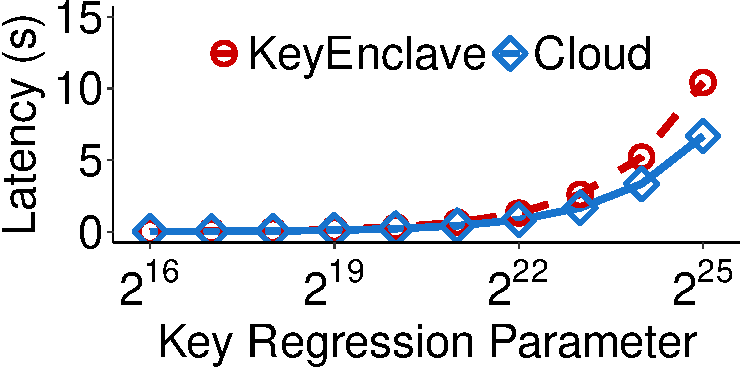
\includegraphics[width=0.48\textwidth]{pic/sgxdedup/expa5_keyRegression_time.pdf} &
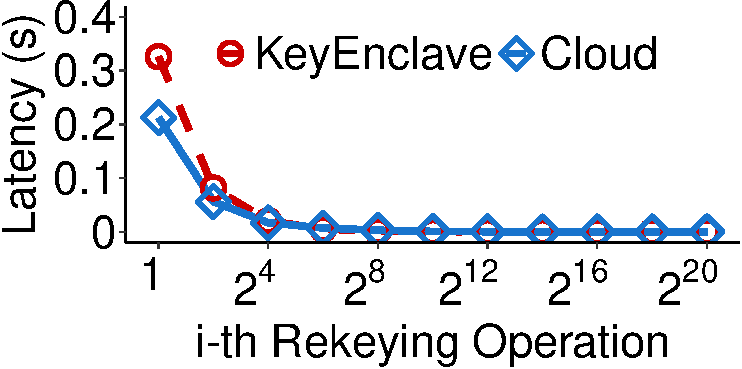
\includegraphics[width=0.48\textwidth]{pic/sgxdedup/expa5_keyRegression_time_default.pdf} \\
\mbox{\small (a) For different parameters} &
\mbox{\small (b) For different occurrences}
\end{tabular}
\caption{(Exp\#12) Rekeying latencies.}
\label{fig:rekeyingLatency}
\end{figure}
